\section{Einleitung}
\subsection{Motivation}
\begin{frame}
\frametitle{Motivation}
\begin{itemize}
\item Große Anwendungsbreite von organischen Halbleitern
\item Polyacetylen als einfaches Testsystem
\item 1950-er \textsc{Longuet-Higgins}: Alternierende Bindungslängen
\item 1980-er \textsc{Su, Schrieffer, Heeger}: Anregungen (Soliton)
\item Gute Bandstruktur mit Tight-Binding
\end{itemize}

\centering
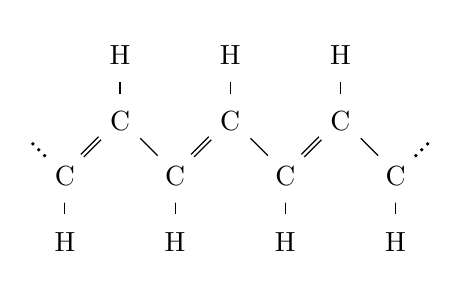
\begin{tikzpicture}[scale = .7]
		\foreach \i in {0,2,4}{
			\draw (\i, 0) -- +(1,1);
			\draw (\i, 0.1) -- +(1,1);
			\draw (\i + 1, 1.05) -- +(1, -1);
			\draw (\i, 0) -- +(0,-.7) node[circle, fill = white, below] {H};
			\draw (\i + 1, 1) -- +(0,.7) node[circle, fill = white, above] {H};
			\node[circle, fill = white] (d\i) at (\i, 0) {C};
			\node[circle, fill = white] (u\i) at (\i + 1, 1) {C};
			}
		\draw (6, 0) -- +(0,-.7) node[circle, fill = white, below] {H};
		\node[circle, fill = white] (end) at (6,0) {C};
		\draw [dotted, line width = 1] (end) -- +(.65,.65);
		\draw [dotted, line width = 1] (d0) -- +(-.65,.65);
\end{tikzpicture}
\end{frame}

\subsection{Dichtefunktionaltheorie}
\begin{frame}
\frametitle{Dichtefunktionaltheorie}
\begin{itemize}
\item Numerische, ab initio, Selbstkonsistenz-Methode zur Berechnung von quantenmechanischen Grundzuständen
\item \textsc{Born-Oppenheimer}-Näherung
\item \textsc{Hohenberg-Kohn} Theoreme:\\
Elektronendichte des Grundzustands bestimmt externes Potential eindeutig und damit Grundzustands-Wellenfunktion:
\begin{align*}
\Psi_0 &= \Psi\left[n_0\right]
\end{align*}
Die Grundzustandsdichte minimiert das Energie-Funktional:
\begin{align*}
E[n_0] &\le E[n]
\end{align*}
\end{itemize}
\end{frame}

\begin{frame}
\begin{itemize}
\item Nicht wechselwirkende Elektron-Wellenfunktionen $\varphi_i$  (\textsc{Kohn-Sham}-Orbitale) mit selber Elektronendichte
\begin{align*}
n(\vec{r}) &= \sum_i \left|\varphi_i\right|^2
\end{align*}
und Einteilchen-Hamiltonian:
\begin{align*}
\mathcal{H} &= \frac{\vec{p}^2}{2m} + V_\text{eff}(\vec{r}, n(\vec{r}))
\end{align*}
\end{itemize}

\end{frame}


\subsection{Constrained Density Functional Theory}
\begin{frame}{}
\end{frame}